% Options for packages loaded elsewhere
\PassOptionsToPackage{unicode}{hyperref}
\PassOptionsToPackage{hyphens}{url}
%
\documentclass[
]{article}
\usepackage{lmodern}
\usepackage{amsmath}
\usepackage{ifxetex,ifluatex}
\ifnum 0\ifxetex 1\fi\ifluatex 1\fi=0 % if pdftex
  \usepackage[T1]{fontenc}
  \usepackage[utf8]{inputenc}
  \usepackage{textcomp} % provide euro and other symbols
  \usepackage{amssymb}
\else % if luatex or xetex
  \usepackage{unicode-math}
  \defaultfontfeatures{Scale=MatchLowercase}
  \defaultfontfeatures[\rmfamily]{Ligatures=TeX,Scale=1}
\fi
% Use upquote if available, for straight quotes in verbatim environments
\IfFileExists{upquote.sty}{\usepackage{upquote}}{}
\IfFileExists{microtype.sty}{% use microtype if available
  \usepackage[]{microtype}
  \UseMicrotypeSet[protrusion]{basicmath} % disable protrusion for tt fonts
}{}
\makeatletter
\@ifundefined{KOMAClassName}{% if non-KOMA class
  \IfFileExists{parskip.sty}{%
    \usepackage{parskip}
  }{% else
    \setlength{\parindent}{0pt}
    \setlength{\parskip}{6pt plus 2pt minus 1pt}}
}{% if KOMA class
  \KOMAoptions{parskip=half}}
\makeatother
\usepackage{xcolor}
\IfFileExists{xurl.sty}{\usepackage{xurl}}{} % add URL line breaks if available
\IfFileExists{bookmark.sty}{\usepackage{bookmark}}{\usepackage{hyperref}}
\hypersetup{
  pdftitle={Title of Your Submission},
  pdfauthor={Jane Doe, MD, MPH1; John Doe, MD, MBI2},
  hidelinks,
  pdfcreator={LaTeX via pandoc}}
\urlstyle{same} % disable monospaced font for URLs
\usepackage[margin=1in]{geometry}
\usepackage{longtable,booktabs}
\usepackage{calc} % for calculating minipage widths
% Correct order of tables after \paragraph or \subparagraph
\usepackage{etoolbox}
\makeatletter
\patchcmd\longtable{\par}{\if@noskipsec\mbox{}\fi\par}{}{}
\makeatother
% Allow footnotes in longtable head/foot
\IfFileExists{footnotehyper.sty}{\usepackage{footnotehyper}}{\usepackage{footnote}}
\makesavenoteenv{longtable}
\usepackage{graphicx}
\makeatletter
\def\maxwidth{\ifdim\Gin@nat@width>\linewidth\linewidth\else\Gin@nat@width\fi}
\def\maxheight{\ifdim\Gin@nat@height>\textheight\textheight\else\Gin@nat@height\fi}
\makeatother
% Scale images if necessary, so that they will not overflow the page
% margins by default, and it is still possible to overwrite the defaults
% using explicit options in \includegraphics[width, height, ...]{}
\setkeys{Gin}{width=\maxwidth,height=\maxheight,keepaspectratio}
% Set default figure placement to htbp
\makeatletter
\def\fps@figure{htbp}
\makeatother
\setlength{\emergencystretch}{3em} % prevent overfull lines
\providecommand{\tightlist}{%
  \setlength{\itemsep}{0pt}\setlength{\parskip}{0pt}}
\setcounter{secnumdepth}{-\maxdimen} % remove section numbering
\usepackage{booktabs}
\usepackage{longtable}
\usepackage{array}
\usepackage{multirow}
\usepackage{wrapfig}
\usepackage{float}
\usepackage{colortbl}
\usepackage{pdflscape}
\usepackage{tabu}
\usepackage{threeparttable}
\usepackage{threeparttablex}
\usepackage[normalem]{ulem}
\usepackage{makecell}
\usepackage{xcolor}
\ifluatex
  \usepackage{selnolig}  % disable illegal ligatures
\fi
\newlength{\cslhangindent}
\setlength{\cslhangindent}{1.5em}
\newlength{\csllabelwidth}
\setlength{\csllabelwidth}{3em}
\newenvironment{CSLReferences}[3] % #1 hanging-ident, #2 entry spacing
 {% don't indent paragraphs
  \setlength{\parindent}{0pt}
  % turn on hanging indent if param 1 is 1
  \ifodd #1 \everypar{\setlength{\hangindent}{\cslhangindent}}\ignorespaces\fi
  % set entry spacing
  \ifnum #2 > 0
  \setlength{\parskip}{#2\baselineskip}
  \fi
 }%
 {}
\usepackage{calc}
\newcommand{\CSLBlock}[1]{#1\hfill\break}
\newcommand{\CSLLeftMargin}[1]{\parbox[t]{\csllabelwidth}{#1}}
\newcommand{\CSLRightInline}[1]{\parbox[t]{\linewidth - \csllabelwidth}{#1}}
\newcommand{\CSLIndent}[1]{\hspace{\cslhangindent}#1}

\title{\textbf{Title of Your Submission}}
\author{Jane Doe, MD, MPH\textsuperscript{1} \and John Doe, MD, MBI\textsuperscript{2}}
\date{}

\begin{document}
\maketitle

\textsuperscript{1} Institution, City, State, Country\\
\textsuperscript{2} Institution, City, State, Country

\hypertarget{what-might-the-attendee-be-able-to-do-after-being-in-your-session}{%
\subsection{What might the attendee be able to do after being in your session?}\label{what-might-the-attendee-be-able-to-do-after-being-in-your-session}}

This section should describe what the attendee might be able to do with the knowledge you are sharing. ``Clinical'' is part of this meeting's name, and ``Best Practices'' is a pillar of the AMIA 2020 Clinical Informatics Conference. This short statement of 1 - 2 sentences is your opportunity to tell attendees the practical implications of your findings on what clinical informaticians do, or on patient/population outcomes

\hypertarget{description-of-the-problem-or-gap}{%
\subsection{Description of the Problem or Gap}\label{description-of-the-problem-or-gap}}

Define the problem or gap here. EG, what HIT tool is poorly designed, or non-existent, or creating barriers to better clinician performance or patient/population outcomes?

Please use this format for reference citations\textsuperscript{\protect\hyperlink{ref-pryor_help_1983}{1},\protect\hyperlink{ref-gardner_computer-critiqued_1990}{2}}.

\hypertarget{methods-what-did-you-do-to-address-the-problem-or-gap}{%
\subsection{Methods: What did you do to address the problem or gap?}\label{methods-what-did-you-do-to-address-the-problem-or-gap}}

This text uses a paragraph to describe methods.

\hypertarget{results-what-was-the-outcomes-of-what-you-did-to-address-the-problem-or-gap}{%
\subsection{Results: What was the outcome(s) of what you did to address the problem or gap?}\label{results-what-was-the-outcomes-of-what-you-did-to-address-the-problem-or-gap}}

This is a write-up of your results.

Use the examples below if you will include a figure or a table. Figures need to be placed as close to the corresponding text as possible and not extend beyond one page. See Figure \ref{fig:nice-fig}.

\begin{figure}

{\centering 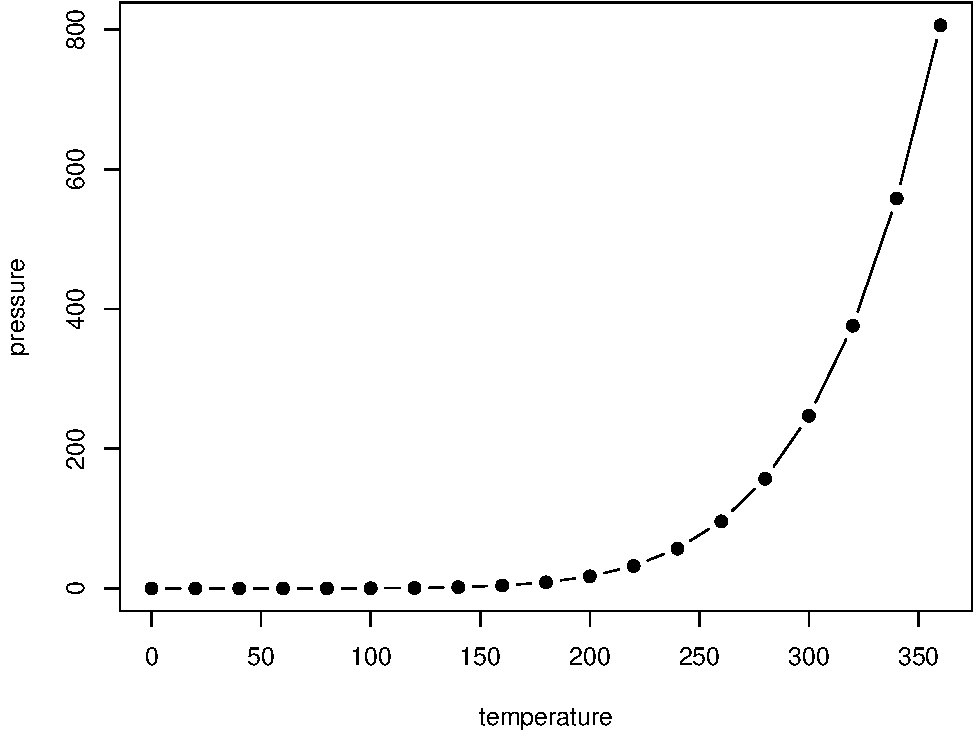
\includegraphics[width=0.5\linewidth]{testmanuscript_files/figure-latex/nice-fig-1} 

}

\caption{Here is a nice figure!}\label{fig:nice-fig}
\end{figure}

This paragraph contains a reference to Table \ref{tab:nice-tab} below. This table contains information on word and page limits per meeting format submission abstract; \textcolor{red}{if your submission is longer than what is specified, it will be rejected without review.} All tables need to be placed as close to the corresponding text as possible, but each individual table should be on one page and not extend to multiple pages unless labeled as ``Continued.'' All submissions must have a brief abstract (word limit as in Table \ref{tab:nice-tab}. The abstract is NOT part of this submission document. You must enter the abstract on the ScholarOne submission website in the Abstract box in Step 1 of your submission process. If your submission is accepted, this abstract is used in our meeting materials, so be sure that it clearly and briefly describes your work

\begin{table}

\caption{\label{tab:nice-tab}Submission type, abstract length, and page length maximum for AMIA submissions.}
\centering
\begin{tabular}[t]{lll}
\toprule
Submission Type & Abstract Length & Page Length Maximum\\
\midrule
Workshop & 250-300 words & Four\\
Presentation & 50-75 words & Two*\\
Panel & 150-200 words & Three\\
Poster & 50-75 words & One\\
Ignite-style Talk & 50-75 words & One\\
\bottomrule
\multicolumn{3}{l}{\rule{0pt}{1em}\textsuperscript{*} Tables and figures go on page 2}\\
\end{tabular}
\end{table}

\hypertarget{discussion-of-results}{%
\subsection{Discussion of Results}\label{discussion-of-results}}

This text uses a paragraph to describe important findings of the project. This text uses a paragraph to describe important findings of the project. This text uses a paragraph to describe important findings of the project. This text uses a paragraph to describe important findings of the project.

\hypertarget{conclusion}{%
\subsection{Conclusion}\label{conclusion}}

Your conclusion goes at the end, followed first by Attendee's Take-away Tool, then followed by References, which must follow the \href{http://www.citethisforme.com/}{Vancouver Style}.

\hypertarget{attendees-take-away-tool}{%
\subsection{Attendee's Take-away Tool}\label{attendees-take-away-tool}}

This text describes the take-away tool. This may be a strategy, an algorithm, an app, etc. The ``tool'' is what the attendee can use to reproduce your study in his/her own practice setting. The presenter may use an illustration to depict the tool on the 2nd page of the submission abstract.

\hypertarget{use-of-knowledge-acquired-at-previous-amia-events}{%
\subsection{Use of Knowledge Acquired at Previous AMIA Events}\label{use-of-knowledge-acquired-at-previous-amia-events}}

Did something you learned at a previous AMIA event contribute to your awareness of the problem or to the solution or strategy you describe in this submission? If so, mention it here. This section may go over to an additional page and will not be counted against you if you have this as an extra page in the page count.

\href{https://www.amia.org/sites/default/files/CIC2021-Submission-Template.pdf}{Original document here}. I have made some stylistic changes that I believe are appropriate for modern formatting.

\hypertarget{references}{%
\subsection*{References}\label{references}}
\addcontentsline{toc}{subsection}{References}

\hypertarget{refs}{}
\begin{CSLReferences}{0}{0}
\leavevmode\hypertarget{ref-pryor_help_1983}{}%
1. Pryor TA, Gardner RM, Clayton PD, Warner HR. The {HELP} system {[}Internet{]}. Journal of Medical Systems. 1983 Apr. ;7(2):87--102.{[}cited 2021 Jan. 8{]} Available from: \url{https://doi.org/10.1007/BF00995116}

\leavevmode\hypertarget{ref-gardner_computer-critiqued_1990}{}%
2. Gardner RM, Golubjatnikov OK, Laub RM, Jacobson JT, Evans RS. Computer-critiqued blood ordering using the {HELP} system {[}Internet{]}. Computers and Biomedical Research. 1990 Dec. ;23(6):514--528.{[}cited 2021 Jan. 8{]} Available from: \url{https://www-sciencedirect-com.ezp-prod1.hul.harvard.edu/science/article/pii/001048099090038E}

\end{CSLReferences}

\end{document}
